% =============================================================================
% Plantilla de paper — Laboratorio 4: Capa de Red (OMNeT++)
% Cátedra de Redes y Sistemas Distribuidos — FaMAF/UNC
%
% Compilación:
%   pdflatex lab4-paper.tex
%   pdflatex lab4-paper.tex
%
% Carpeta figuras/: coloque ahí PDF/PNG exportados desde OMNeT++ o scripts.
% Antes de entregar: elimine todas las cajas \guia{...} y reemplace los
% textos de ejemplo por su contenido definitivo. Objetivo final: 6 a 8 páginas.
% =============================================================================

\documentclass[10pt,letterpaper,twocolumn]{article}

\usepackage[T1]{fontenc}
\usepackage[utf8]{inputenc}
\usepackage[english]{babel}
\usepackage[margin=0.9in]{geometry}
\usepackage{amsmath,amsfonts}
\usepackage{graphicx}
\usepackage{booktabs}
\usepackage{multirow}
\usepackage{subcaption}
\usepackage{xcolor}
\usepackage{url}
\usepackage[hidelinks]{hyperref}
\usepackage{tikz}
\usepackage{pgfplots}
\pgfplotsset{compat=1.18}
\usetikzlibrary{arrows.meta}

% ---------------------------------------------------------------------------
% Caja de instrucciones para el alumno (eliminar antes de la entrega final)
% ---------------------------------------------------------------------------
\newcommand{\guia}[1]{%
  \par\smallskip\noindent
  \fcolorbox{blue!60!black}{blue!4}{%
    \parbox{\dimexpr\linewidth-2\fboxsep-2\fboxrule}{%
      \small
      \textbf{\textcolor{blue!60!black}{Guía para completar:}}~#1
    }%
  }%
  \smallskip\par
}

% Tablas que deben caber dentro de una columna (formato 2 columnas)
\newcommand{\coltablesetup}{%
  \scriptsize
  \setlength{\tabcolsep}{3pt}%
  \renewcommand{\arraystretch}{1.08}%
}

% Datos del grupo — modifique estos campos
\newcommand{\Titulo}{Routing Strategies for Ring Topologies in OMNeT++}
\newcommand{\Grupo}{Grupo 23}
\newcommand{\Integrantes}{Álvarez, Lis Ailín; Pinilla, Lautaro; Sabino, Lucas}
\renewcommand{\refname}{Referencias}
\renewcommand{\abstractname}{Abstract}
\renewcommand{\appendixname}{Ap\'{e}ndice}

% Entorno estilo revista para metadatos en inglés
\newenvironment{IEEEkeywords}{%
  \smallskip\noindent\textbf{Index Terms---}%
}{\par\smallskip}

\begin{document}

\twocolumn[
\begin{@twocolumnfalse}
  \begin{center}
    {\LARGE\bfseries \Titulo\par}
    \vspace{0.6em}
    {\normalsize \Integrantes\par}
    \vspace{0.4em}
    {\small \Grupo, Facultad de Matemática, Astronomía, Física y Computación (FaMAF)\\
    Universidad Nacional de Córdoba, Argentina\par}
    \vspace{1em}
  \end{center}

  \begin{abstract}
  \noindent
  This paper evaluates a baseline routing algorithm in an OMNeT++ ring network of 8 nodes, which forwards all packets through a fixed interface. Two traffic scenarios are analyzed: two sources and seven sources sending to node~5, with varying inter-arrival times. Metrics include delay, hop count, buffer occupancy, and link utilization. The baseline shows asymmetric load, long delays, and a stability threshold near 7~s, below which queues grow indefinitely. To overcome this, we propose a distance-based algorithm using both ring directions, discovering the network size autonomously via an initial exchange of hello and echo messages without OMNeT++ topology functions. Our algorithm selects the shortest path, balances traffic, and avoids loops. Results show significant reductions in delay and buffer usage, and a higher stability threshold (from $IAT > 7$\,s to $IAT > 4$\,s theoretically). The design scales to any ring size through this neighbor discovery mechanism. No routing loops were observed.
  \end{abstract}

  \begin{IEEEkeywords}
  Network simulation, OMNeT++, routing, ring topology, performance evaluation,
  queueing, stability.
  \end{IEEEkeywords}

\end{@twocolumnfalse}
]

\selectlanguage{english}
% Contenido principal en español (sin babel-spanish; títulos de sección en español manualmente)

\section{Introducción}
\label{sec:intro}

Este artículo reporta el análisis y diseño de estrategias de enrutamiento
implementadas sobre el modelo de red del Laboratorio~4. Se estudia una red
en anillo de ocho nodos en la que el algoritmo baseline reenvía siempre los
paquetes por la misma interfaz (\texttt{toLnk[0]}), sin aprovechar el camino
alternativo disponible. El objetivo es instrumentar métricas de desempeño,
incluyendo demora, cantidad de saltos, ocupación de buffers y utilización de
enlaces, evaluar el comportamiento del algoritmo baseline en distintos
escenarios de tráfico y diseñar una estrategia de enrutamiento mejorada. El
trabajo se organiza de la siguiente manera: la Sección~\ref{sec:modelo}
describe el modelo de simulación; la Sección~\ref{sec:baseline} presenta el
análisis del algoritmo baseline; la Sección~\ref{sec:nuevo} detalla el diseño
del nuevo algoritmo; la Sección~\ref{sec:comparacion} compara los resultados
obtenidos; y finalmente la Sección~\ref{sec:conclusiones} resume las
conclusiones del trabajo.

La principal limitación del baseline es el uso exclusivo de una de las dos
interfaces, lo que satura un sentido del anillo mientras el otro permanece
vacío. Esto provoca demoras innecesarias, buffers largos y baja eficiencia.
Una estrategia será considerada mejor si reduce la demora media, equilibra la
carga entre ambas direcciones, evita bucles y permite sostener tasas de
tráfico más altas antes de la saturación.

Se propone un algoritmo de enrutamiento por distancia mínima que utiliza ambos
sentidos del anillo, descubriendo la topología mediante mensajes hello. De
esta forma, cada paquete sigue el camino más corto al destino. Se espera una
mejora significativa en demora, balance de carga y umbral de estabilidad
respecto del baseline, sin introducir bucles de enrutamiento.

\section{Escenario y modelo de simulación}
\label{sec:modelo}

La topología utilizada es un anillo de 8 nodos numerados del 0 al 7. Cada nodo posee dos interfaces full-duplex (denominadas \texttt{lnk[0]} y \texttt{lnk[1]}) que lo conectan con sus dos vecinos. Internamente, cada nodo se compone de tres submódulos: la capa de aplicación (\texttt{app}), que genera paquetes según una distribución exponencial con tamaño fijo; la capa de red (\texttt{net}), que implementa la lógica de enrutamiento; y dos capas de enlace (\texttt{lnk[0]} y \texttt{lnk[1]}), cada una con su propio buffer y un servidor que modela la transmisión a 1~Mbps con un retardo de propagación de 100~$\mu$s. La Figura~\ref{fig:topologia} muestra la disposición de la red.

\begin{figure}[!ht]
  \centering
  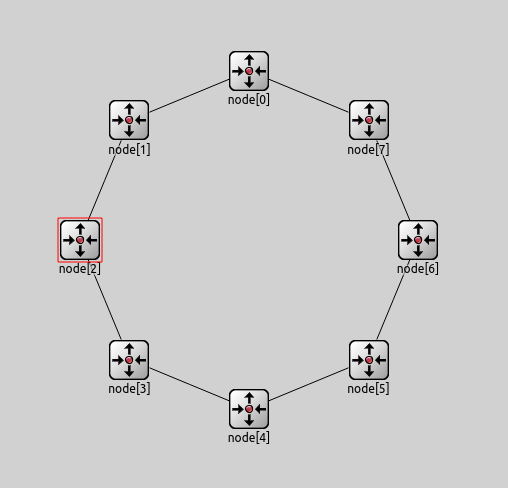
\includegraphics[width=0.8\linewidth]{figuras/network.png}
  \caption{Topología en anillo de 8 nodos.}
  \label{fig:topologia}
\end{figure}

\subsection{Topología y configuración de tráfico}

Todos los enlaces son full-duplex, con capacidad de 1~Mbps y retardo de propagación de 100~$\mu$s. La capa de aplicación genera paquetes de 125000 bytes con tiempos entre llegadas exponenciales. En el \textbf{Caso 1}, solo los nodos 0 y 2 actúan como fuentes, ambos con destino en el nodo 5 y una tasa media de 1 paquete por segundo (\texttt{exponential(1)}). En el \textbf{Caso 2}, todos los nodos excepto el 5 (es decir, los nodos 0,1,2,3,4,6,7) generan tráfico hacia el nodo 5, y se varía el valor de \texttt{interArrivalTime} en el rango de 0.5 a 8 segundos (específicamente: 0.5, 1, 2, 4, 6, 8) para estudiar la estabilidad. La Tabla~\ref{tab:config} resume los parámetros empleados.

\begin{table}[!ht]
  \centering
  \caption{Configuración experimental por escenario.}
  \label{tab:config}
  \coltablesetup
  \resizebox{\columnwidth}{!}{%
  \begin{tabular}{@{}lccc@{}}
    \toprule
    \textbf{Parámetro} & \textbf{Caso 1} & \textbf{Caso 2} & \textbf{Comp.} \\
    \midrule
    Fuentes activas & \texttt{n[0]}, \texttt{n[2]} & 7 $\to$ \texttt{n[5]} & 1 y 2 \\
    Destino & \texttt{n[5]} & \texttt{n[5]} & idem \\
    \texttt{packetByteSize} & 125000 bytes & 125000 bytes & 125000 bytes \\
    \texttt{interArrivalTime} & \texttt{exponential(1)} & \texttt{exponential(0.5 a 8)} & -- \\
    T. simulación (s) & 200 & 200 & 200 \\
    Semilla & 1 & 1 & 1 \\
    \bottomrule
  \end{tabular}%
  }
\end{table}

\subsection{Métricas registradas}
Para evaluar el rendimiento del sistema de enrutamiento se instrumentaron las siguientes métricas en los módulos correspondientes:
\begin{itemize}
    \item \textbf{Demora extremo a extremo (s)}: medida en la capa de aplicación del nodo destino, calculando la diferencia entre el tiempo de recepción y el de creación del paquete.
    \item \textbf{Cantidad de saltos por paquete}: se incrementa un contador en la capa de red de cada nodo que reenvía el paquete; el valor final se registra en la aplicación destino.
    \item \textbf{Ocupación de buffer (paquetes)}: se registra la longitud instantánea de la cola en cada capa de enlace cada vez que se encola o desencola un paquete.
    \item \textbf{Utilización del enlace (\%)}: se acumula el tiempo total de transmisión de paquetes en cada interfaz y se divide por el tiempo total de simulación.
\end{itemize}

La Tabla~\ref{tab:metricas} resume las métricas y sus módulos.

\begin{table}[!ht]
  \centering
  \caption{Métricas instrumentadas en el simulador.}
  \label{tab:metricas}
  \coltablesetup
  \resizebox{\columnwidth}{!}{%
  \begin{tabular}{@{}lcc@{}}
    \toprule
    \textbf{Métrica} & \textbf{Módulo} & \textbf{Unid.} \\
    \midrule
    Demora E2E (promedio) & \texttt{app} & s \\
    Paquetes enviados & \texttt{app} & adim. \\
    Paquetes recibidos & \texttt{app} & adim. \\
    Saltos por paquete (promedio) & \texttt{app} & adim. \\
    Saltos por paquete (máximo) & \texttt{app} & adim. \\
    Ocupación buffer (promedio) & \texttt{lnk} & pkts \\
    Ocupación buffer (máximo) & \texttt{lnk} & pkts \\
    Utilización enlace & \texttt{lnk} & \% \\
    \bottomrule
  \end{tabular}%
  }
\end{table}

\section{Tarea de análisis: evaluación del kickstarter}
\label{sec:analisis}

En esta sección se presenta la evaluación de rendimiento del algoritmo 
de enrutamiento base (kickstarter) implementado en la topología de anillo. 
Para diagnosticar sus limitaciones, el análisis se divide en dos escenarios 
de simulación. El Caso 1 evalúa el comportamiento y la distribución de 
carga de la red ante fuentes específicas (\texttt{node[0]} y \texttt{node[2]} hacia \texttt{node[5]}). Dado que el algoritmo reenvía siempre los paquetes por la interfaz \texttt{toLnk[0]}, el tráfico se ve forzado a viajar invariablemente en sentido antihorario (\texttt{2} $\to$ \texttt{1} $\to$ \texttt{0} $\dots$ $\to$ \texttt{5}), adoptando rutas que no siempre son óptimas.
Por su parte, el Caso 2 busca determinar el punto de saturación de los 
buffers frente a un incremento generalizado y sostenido del tráfico. 
Las métricas obtenidas en ambos experimentos servirán como línea base 
empírica para justificar el diseño de un algoritmo de enrutamiento mejorado.

\subsection{Caso 1: tráfico configurado (\texttt{node[0]} y \texttt{node[2]} $\rightarrow$ \texttt{node[5]})}
\label{sec:baseline}

En esta simulación, evaluamos el desempeño de la red bajo un escenario asimétrico, donde solo \texttt{node[0]} y \texttt{node[2]} generan tráfico hacia \texttt{node[5]}. Según los resultados resumidos en la Tabla~\ref{tab:caso1}, el algoritmo baseline obtiene una demora media de 53.25\,s, lo cual evidencia una congestión importante. En cuanto al uso de recursos, se observó que la ocupación máxima a nivel global alcanzó los 199 paquetes y la utilización máxima de enlace llegó al 98\%, demostrando que prácticamente el enlace en la dirección de transmisión elegida por el enrutamiento estático está saturado.

Al analizar el tráfico de forma individual (ver Fig.~\ref{fig:caso1-demora}), se hace evidente el problema estructural del algoritmo baseline: el flujo de tráfico estático hace que el \texttt{node[0]} absorba tanto los paquetes generados por él mismo, como los que arriban desde y a través del \texttt{node[2]} (en su camino hacia el \texttt{node[5]}). Esto transforma al \texttt{node[0]} e indirectamente sus puertos \texttt{lnk[0]} en un cuello de botella crítico (con un buffer que llega al tope de 199 paquetes y en 98\% utilización de enlace), mientras que los recursos propios iniciales de \texttt{node[2]} tienen menor presión.

Como consecuencia directa de esta congestión, surge una penalización generalizada e ineficiente en las demoras. Mientras que el tráfico de la Fuente 2 requiere 5 saltos para llegar a destino, la Fuente 0 solo requiere 3. Sin embargo, las demoras promedio son extremadamente similares (en torno a los 53\textendash 54\,s para ambas). Esto demuestra que el tiempo extra de transmisión por dar más saltos termina siendo insignificante comparado con el masivo retraso que ambos flujos sufren (queueing delay) al quedar atascados en la misma cola del nodo saturado (\texttt{node[0]}), haciendo que los paquetes tarden prácticamente lo mismo en llegar al destino sin importar su punto de partida.

Este cuello de botella y las demoras asociadas subrayan la necesidad de implementar esquemas de ruteo basados en métricas de distancia que balanceen la carga de red por ambos sentidos del anillo (para ir por el camino más corto).


\begin{table}[!ht]
  \centering
  \caption{Resultados globales del Caso~1 (baseline).}
  \label{tab:caso1}
  \coltablesetup
  \resizebox{\columnwidth}{!}{%
  \begin{tabular}{@{}lrrr@{}}
    \toprule
    \textbf{Métrica} & \textbf{Prom.} & \textbf{Máx.} & \textbf{Desv.} \\
    \midrule
    Demora (s)        & 53.25 & -- & -- \\
    Saltos            & 3.8  & 5    & 0.98  \\
    Ocupación buffer  & 21.8  & 199    & 43.4  \\
    Util. enlace (\%) & 29.5  & 98.0  & 45.2  \\
    \bottomrule
  \end{tabular}%
  }
\end{table}

\begin{figure}[!t]
  \centering
  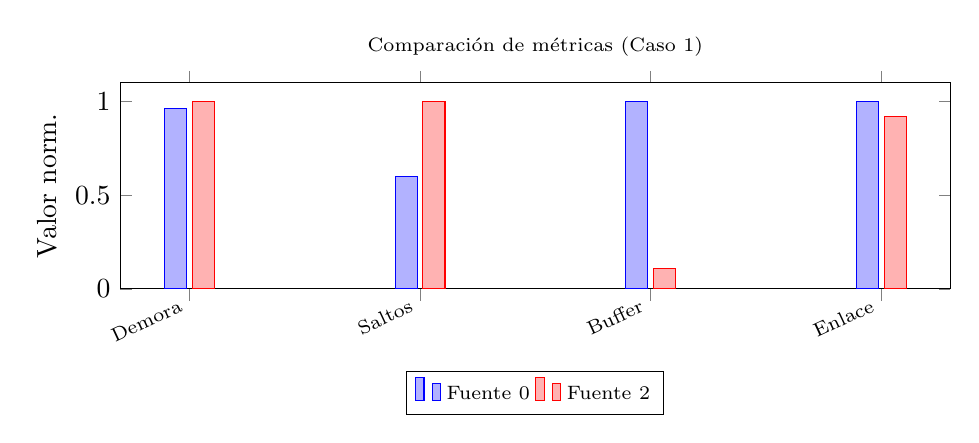
\begin{tikzpicture}
    \begin{axis}[
      width=\linewidth,
      height=4.2cm,
      ybar,
      bar width=8pt,
      ymin=0,
      symbolic x coords={Demora,Saltos,Buffer,Enlace},
      xtick=data,
      x tick label style={font=\scriptsize, rotate=25, anchor=east},
      ylabel={Valor norm.},
      title={\scriptsize Comparación de métricas (Caso 1)},
      legend style={font=\scriptsize, at={(0.5,-0.40)}, anchor=north, legend columns=-1},
    ]
      \addplot coordinates {(Demora,0.96) (Saltos,0.60) (Buffer,1.00) (Enlace,1.00)};
      \addplot coordinates {(Demora,1.00) (Saltos,1.00) (Buffer,0.11) (Enlace,0.92)};
      \legend{Fuente 0, Fuente 2}
    \end{axis}
  \end{tikzpicture}
  \caption{Métricas normalizadas para el Caso 1 (baseline). La métrica Buffer (máximo) y Enlace correlacionan los nodos \texttt{node[0]} para Fuente 0 y \texttt{node[2]} para Fuente 2.}
  \label{fig:caso1-demora}
\end{figure}

\subsection{Caso 2: tráfico sostenido hacia \texttt{node[5]}}
\label{sec:caso2}

En este escenario los siete nodos restantes del anillo
(\texttt{node[0]}--\texttt{node[4]}, \texttt{node[6]} y \texttt{node[7]})
generan tráfico simultáneamente hacia \texttt{node[5]} con el mismo
\texttt{packetByteSize} (125\,000 bytes $=1$\,Mbit) e
\texttt{interArrivalTime} exponencial. Se exploraron seis valores: 0.5, 1,
2, 4, 6 y 8 segundos, con el objetivo de determinar el umbral de
estabilidad de la red bajo el algoritmo baseline.

\subsubsection*{Dirección del tráfico y cuello de botella}

El archivo \texttt{.ned} define las conexiones del anillo de la siguiente
manera:

\begin{small}
\begin{verbatim}
node[0].toNod[1] <--> node[1].toNod[0]
node[1].toNod[1] <--> node[2].toNod[0]
...
node[7].toNod[1] <--> node[0].toNod[0]
\end{verbatim}
\end{small}

\noindent El módulo \texttt{Net} del baseline reenvía siempre por
\texttt{toLnk[0]}, que corresponde a \texttt{toNod[0]}. Dado que
\texttt{toNod[0]} de cada nodo $n$ está conectado a \texttt{toNod[1]} del
nodo $n-1$, los paquetes viajan en dirección \textbf{decreciente}:
$n \to n{-}1 \to \cdots \to 5$. Los nodos 6 y 7 quedan al otro lado del
destino, por lo que recorren el camino largo:
$6\to5$ (1 salto) y $7\to6\to5$ (2 saltos), mientras que el
\texttt{node[4]} debe atravesar todo el anillo ($4\to3\to\cdots\to6\to5$,
7 saltos). La Tabla~\ref{tab:flujos} resume los flujos acumulados
en cada enlace.

\begin{table}[!ht]
  \centering
  \caption{Flujos acumulados por enlace bajo routing baseline
           (dirección decreciente, destino \texttt{node[5]}).}
  \label{tab:flujos}
  \coltablesetup
  \resizebox{\columnwidth}{!}{%
  \begin{tabular}{@{}lcc@{}}
    \toprule
    \textbf{Enlace} & \textbf{Flujos} & \textbf{Nodos que transitan} \\
    \midrule
    \texttt{node[4].lnk[0]} & 1 & \texttt{n[4]} \\
    \texttt{node[3].lnk[0]} & 2 & \texttt{n[4]}, \texttt{n[3]} \\
    \texttt{node[2].lnk[0]} & 3 & \texttt{n[4]}--\texttt{n[2]} \\
    \texttt{node[1].lnk[0]} & 4 & \texttt{n[4]}--\texttt{n[1]} \\
    \texttt{node[0].lnk[0]} & 5 & \texttt{n[4]}--\texttt{n[0]} \\
    \texttt{node[7].lnk[0]} & 6 & \texttt{n[4]}--\texttt{n[7]} \\
    \texttt{node[6].lnk[0]} & 7 & todos \\
    \bottomrule
  \end{tabular}%
  }
\end{table}

El enlace \texttt{node[6].lnk[0]} concentra los 7 flujos y constituye el
cuello de botella teórico. Su utilización es:

\begin{equation}
  \rho = \frac{7}{\mathrm{IAT}} \times T_s
       = \frac{7}{\mathrm{IAT}} \times 1\,\mathrm{s}
       = \frac{7}{\mathrm{IAT}}
  \label{eq:rho}
\end{equation}

\noindent donde $T_s = 1\,\mathrm{Mbit}/1\,\mathrm{Mbps} = 1\,\mathrm{s}$
es el tiempo de servicio. La condición de estabilidad $\rho < 1$ exige:

\begin{equation}
  \mathrm{IAT} > 7\,\mathrm{s}
  \label{eq:umbral}
\end{equation}

\subsubsection*{Resultados experimentales}

La Tabla~\ref{tab:caso2-sweep} resume las métricas medidas. La columna
``R/E'' indica la fracción de paquetes generados que llegaron a destino
durante los 200\,s de simulación.

\begin{table}[!ht]
  \centering
  \caption{Métricas del Caso~2 en función del \texttt{interArrivalTime}.
           BufMáx corresponde a \texttt{node[6].lnk[0]}.}
  \label{tab:caso2-sweep}
  \coltablesetup
  \resizebox{\columnwidth}{!}{%
  \begin{tabular}{@{}rrrrrrr@{}}
    \toprule
    \textbf{IAT (s)} & \textbf{Demora (s)} & \textbf{Enviados} &
    \textbf{Recib.} & \textbf{R/E} &
    \textbf{BufMáx} & \textbf{¿Estable?} \\
    \midrule
    0.5 & 75.09 & 2820 & 199 & 0.071 & 421 & No \\
    1   & 65.92 & 1422 & 199 & 0.140 & 218 & No \\
    2   & 56.52 &  723 & 198 & 0.274 & 102 & No \\
    4   & 39.99 &  364 & 195 & 0.536 &  50 & No \\
    6   & 17.49 &  225 & 188 & 0.836 &  25 & No \\
    8   &  6.19 &  169 & 164 & 0.970 &   4 & Sí \\
    \bottomrule
  \end{tabular}%
  }
\end{table}

Las Figuras~\ref{fig:caso2-estabilidad} y~\ref{fig:caso2-util} muestran
la evolución de la demora media y la utilización de los enlaces más
representativos en función del \texttt{interArrivalTime}.

\begin{figure}[!t]
  \centering
  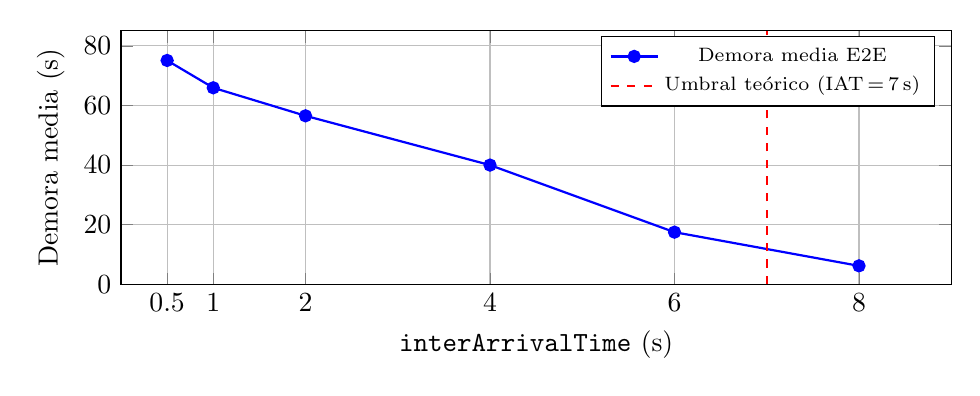
\begin{tikzpicture}
    \begin{axis}[
      width=\linewidth,
      height=4.8cm,
      xlabel={\texttt{interArrivalTime} (s)},
      ylabel={Demora media (s)},
      xmin=0, xmax=9,
      ymin=0, ymax=85,
      grid=major,
      xtick={0.5,1,2,4,6,8},
      legend style={font=\scriptsize, at={(0.98,0.98)}, anchor=north east},
    ]
      \addplot[thick, blue, mark=*, mark size=2pt] coordinates {
        (0.5,75.09)(1,65.92)(2,56.52)(4,39.99)(6,17.49)(8,6.19)
      };
      \addlegendentry{Demora media E2E}
      \addplot[thick, red, dashed] coordinates {(7,0)(7,85)};
      \addlegendentry{Umbral teórico (IAT\,=\,7\,s)}
    \end{axis}
  \end{tikzpicture}
  \caption{Demora media extremo a extremo vs.\ \texttt{interArrivalTime}
           en el Caso~2. La línea discontinua marca el umbral teórico
           $\rho=1$ (Ec.~\ref{eq:umbral}).}
  \label{fig:caso2-estabilidad}
\end{figure}

\begin{figure}[!t]
  \centering
  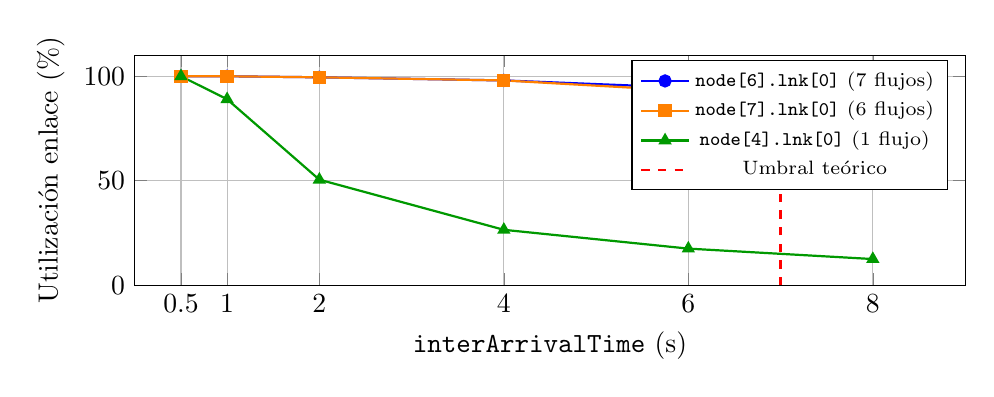
\begin{tikzpicture}
    \begin{axis}[
      width=\linewidth,
      height=4.5cm,
      xlabel={\texttt{interArrivalTime} (s)},
      ylabel={Utilización enlace (\%)},
      xmin=0, xmax=9,
      ymin=0, ymax=110,
      grid=major,
      xtick={0.5,1,2,4,6,8},
      legend style={font=\scriptsize, at={(0.98,0.98)}, anchor=north east},
    ]
      \addplot[thick, blue, mark=*, mark size=2pt] coordinates {
        (0.5,100.0)(1,100.0)(2,99.5)(4,98.0)(6,94.5)(8,82.5)
      };
      \addlegendentry{\texttt{node[6].lnk[0]} (7 flujos)}
      \addplot[thick, orange, mark=square*, mark size=2pt] coordinates {
        (0.5,100.0)(1,100.0)(2,99.5)(4,98.0)(6,93.0)(8,72.0)
      };
      \addlegendentry{\texttt{node[7].lnk[0]} (6 flujos)}
      \addplot[thick, green!60!black, mark=triangle*, mark size=2pt] coordinates {
        (0.5,100.0)(1,89.0)(2,50.5)(4,26.5)(6,17.5)(8,12.5)
      };
      \addlegendentry{\texttt{node[4].lnk[0]} (1 flujo)}
      \addplot[thick, red, dashed] coordinates {(7,0)(7,110)};
      \addlegendentry{Umbral teórico}
    \end{axis}
  \end{tikzpicture}
  \caption{Utilización de enlaces seleccionados vs.\ \texttt{interArrivalTime}.
           \texttt{node[6].lnk[0]} es el cuello de botella (7 flujos);
           \texttt{node[4].lnk[0]} transporta un solo flujo.}
  \label{fig:caso2-util}
\end{figure}

\subsubsection*{Determinación del umbral de estabilidad}

Los datos experimentales confirman que \textbf{la red no es estable para
ningún valor de \texttt{interArrivalTime} $\leq 6$\,s}. Los tres criterios
utilizados para determinar inestabilidad son:

\begin{enumerate}
  \item \textbf{Ratio R/E $\ll 1$}: con IAT\,$=1$\,s solo el 14\,\% de
        los paquetes generados llegan a destino en 200\,s; con
        IAT\,$=6$\,s el ratio sube a 83.6\,\% pero sigue siendo
        significativamente menor que 1.
  \item \textbf{Buffers crecientes}: el buffer máximo de
        \texttt{node[6].lnk[0]} crece de 4 paquetes (IAT\,$=8$\,s)
        a 421 paquetes (IAT\,$=0.5$\,s), sin tender a estabilizarse
        para IAT\,$\leq 6$\,s.
  \item \textbf{Utilización sostenida al límite}: \texttt{node[6].lnk[0]}
        opera al 94.5\,\% con IAT\,$=6$\,s, dejando apenas margen
        ante variaciones aleatorias del tráfico.
\end{enumerate}

Con \texttt{interArrivalTime}\,$=8$\,s se observa el primer régimen
estable: el ratio R/E alcanza 0.970, el buffer máximo del cuello de
botella cae a 4~paquetes, la demora media se reduce a 6.19\,s y la
utilización de \texttt{node[6].lnk[0]} baja al 82.5\,\%. Este resultado
es consistente con el análisis teórico de la
Ecuación~(\ref{eq:umbral}): con IAT\,$=8$\,s se obtiene
$\rho = 7/8 = 0.875 < 1$.

Cabe destacar que la distribución de carga es marcadamente asimétrica.
Los nodos 6 y 7 son los más favorecidos por el routing baseline (1 y 2
saltos respectivamente), mientras que el \texttt{node[4]} recorre 7
saltos para llegar al destino, siendo el más perjudicado. Esta asimetría
estructural, visible en la Fig.~\ref{fig:caso2-util} donde
\texttt{node[4].lnk[0]} tiene apenas 12.5\,\% de utilización frente al
82.5\,\% de \texttt{node[6].lnk[0]}, es consecuencia directa del
algoritmo baseline que ignora la distancia al destino y siempre elige
la misma dirección de reenvío.

\textit{La red garantiza equilibrio a partir de
\texttt{interArrivalTime}\,$=8$\,s, valor consistente con el umbral
teórico $\rho = 7/\mathrm{IAT} < 1$ que exige IAT\,$> 7$\,s
(Ec.~\ref{eq:umbral}).}

\section{Diseño del algoritmo de enrutamiento propuesto}
\label{sec:diseno}

El algoritmo diseñado reemplaza el envío por la misma interfaz \texttt{lnk[0]} por una
decisión basada en la distancia mínima en el anillo. Para ello, cada nodo necesita
conocer la cantidad total de nodos \(N\) y su propio identificador. Esta información
se obtiene sin usar \texttt{cTopology} ni iteradores de \texttt{cGate}, únicamente
mediante el intercambio de dos tipos de paquetes de control: \texttt{hello} y
\texttt{echo}. Una vez que todos los nodos conocen \(N\), el reenvío de cada paquete
de datos se decide calculando la cantidad de saltos en ambos sentidos y eligiendo la
interfaz que da el camino más corto. El diseño es simple, autónomo y se adapta a
cualquier tamaño de anillo, emulando el comportamiento de protocolos reales de
descubrimiento de vecinos.

\subsection{Información disponible y estructuras de datos}

Cada nodo mantiene internamente dos variables globales:
\begin{itemize}
    \item \texttt{totalNodes}: entero que almacena el tamaño del anillo (valor inicial 0).
    \item \texttt{haveTotalNodes}: booleano que indica si un nodo ya se recibió el valor de \texttt{totalNodes}.
\end{itemize}
Además, cada nodo conoce su propio índice (\texttt{nodeId}), obtenido al inicio de la
simulación mediante \texttt{getParentModule()->getIndex()}. No se utilizan tablas
de ruteo explícitas porque la decisión de interfaz se calcula sobre la marcha;
sin embargo, a modo ilustrativo, la Tabla~\ref{tab:rutasfake} muestra cómo se vería la
tabla local de un nodo (por ejemplo, el nodo 4) en un anillo de 8 nodos con nuestro
algoritmo.

\begin{table}[!ht]
  \centering
  \caption{Ejemplo de tabla de rutas locales en el nodo 4 para un anillo de 8 nodos.}
  \label{tab:rutasfake}
  \coltablesetup
  \resizebox{\columnwidth}{!}{%
  \begin{tabular}{@{}clc@{}}
    \toprule
    \textbf{Destino} & \textbf{Interfaz} & \textbf{Saltos} \\
    \midrule
    \texttt{node[5]} & \texttt{lnk[1]} & 1 \\
    \texttt{node[0]} & \texttt{lnk[1]} & 2 \\
    \texttt{node[2]} & \texttt{lnk[1]} & 2 \\
    \texttt{node[6]} & \texttt{lnk[0]} & 2 \\
    \texttt{node[7]} & \texttt{lnk[0]} & 1 \\
    \bottomrule
  \end{tabular}%
  }
\end{table}

Los mensajes de control utilizados tienen los siguientes campos:

\begin{itemize}
    \item \textbf{Mensaje \texttt{hello} (tipo 1)}: se usa para descubrir \(N\).
        \begin{itemize}
            \item \texttt{origin}: nodo que inició el descubrimiento.
            \item \texttt{hopCount}: contador de saltos.
            \item \texttt{packetType} = 1.
        \end{itemize}
    \item \textbf{Mensaje \texttt{echo} (tipo 2)}: propaga el valor de \(N\).
        \begin{itemize}
            \item \texttt{totalNodes}: tamaño del anillo.
            \item \texttt{packetType} = 2.
        \end{itemize}
\end{itemize}

Los paquetes de datos (tipo 0) llevan \texttt{source}, \texttt{destination} y
\texttt{hopCount} (incrementado en cada reenvío).

\subsection{Reglas de decisión}

El algoritmo se divide en dos fases: descubrimiento y enrutamiento. A continuación
se describen en prosa, se proporciona el pseudocódigo y un ejemplo numérico.

\subsubsection*{Descripción en prosa}

\textbf{Fase 1 – Descubrimiento de \(N\):}
\begin{enumerate}
    \item El nodo 0 (elegido arbitrariamente) envía un paquete \texttt{hello} con
        \texttt{hopCount=0} por su interfaz \texttt{lnk[0]}.
    \item Cada nodo intermedio que recibe el \texttt{hello} incrementa
        \texttt{hopCount} y lo reenvía por la misma interfaz \texttt{lnk[0]}.
    \item Cuando el \texttt{hello} regresa al nodo 0, el valor de
        \texttt{hopCount} es el número de saltos (cantidad de nodos intermedios).
        El nodo 0 deduce entonces \texttt{totalNodes = hopCount + 1} y lo almacena.
    \item El nodo 0 construye un paquete \texttt{echo} con \texttt{totalNodes} y lo
        envía por todas sus interfaces conectadas (inundación).
    \item Cada nodo que recibe un \texttt{echo} por primera vez guarda el valor de
        \texttt{totalNodes}, lo reenvía por todas las demás interfaces (excepto por
        la que llegó) y activa la fase de enrutamiento. Los \texttt{echo} duplicados
        se descartan.
\end{enumerate}

\textbf{Fase 2 – Enrutamiento de paquetes de datos:}
\begin{enumerate}
    \item Al recibir un paquete de datos (tipo 0) que no está destinado al nodo local,
        se incrementa su campo \texttt{hopCount}.
    \item Si el nodo aún no conoce \texttt{totalNodes} (fallback), reenvía el paquete
        por \texttt{lnk[0]} (comportamiento baseline).
    \item Si ya conoce \texttt{totalNodes}, calcula las distancias en ambos sentidos:
        \[
        \begin{aligned}
        \mathrm{horario}
            &= (\mathrm{destino} - \mathrm{nodeId} + \mathrm{totalNodes})
            \bmod \mathrm{totalNodes} \\
        \mathrm{antihorario}
            &= (\mathrm{nodeId} - \mathrm{destino} + \mathrm{totalNodes})
            \bmod \mathrm{totalNodes}
        \end{aligned}
        \]
    \item Elige la interfaz según la regla:
        \begin{itemize}
            \item Si \(\text{horario} \le \text{antihorario}\), envía por \texttt{lnk[1]} (sentido horario).
            \item En caso contrario, envía por \texttt{lnk[0]} (sentido antihorario).
        \end{itemize}
\end{enumerate}

\subsubsection*{Pseudocódigo}

\begin{small}
\begin{verbatim}
al recibir paquete p:
  si p.tipo == 1:            # hello
    si p.origen == mi_id:
      totalNodes = p.hopCount + 1
      haveTotalNodes = true
      para cada interfaz i conectada:
        enviar echo(totalNodes) por i
    sino:
      p.hopCount = p.hopCount + 1
      reenviar p por lnk[0]
  si p.tipo == 2:            # echo
    si not haveTotalNodes:
      totalNodes = p.totalNodes
      haveTotalNodes = true
      para cada interfaz i conectada 
                    excepto la de llegada:
        reenviar copia de p por i
  si p.tipo == 0:            # data
    si p.destino == mi_id:
      entregar a app
    sino:
      p.hopCount = p.hopCount + 1
      si not haveTotalNodes:
        reenviar por lnk[0]   # fallback
      sino:
        horario = (p.destino - mi_id + 
                   totalNodes) % totalNodes
        antihorario = (mi_id - p.destino + 
                       totalNodes) % totalNodes
        si horario <= antihorario:
          reenviar por lnk[1]   # horario
        sino:
          reenviar por lnk[0]   # antihorario
\end{verbatim}
\end{small}

\subsubsection*{Ejemplo numérico}

Considere un anillo de 8 nodos (\(N=8\)). El nodo 0 recibe un paquete con
destino al nodo 5. Calcula:

\begin{itemize}
    \item \(\mathrm{horario} = (5 - 0 + 8) \bmod 8 = 5\)

    \item \(\mathrm{antihorario} = (0 - 5 + 8) \bmod 8 = 3\)
\end{itemize}

Dado que \(\mathrm{horario} > \mathrm{antihorario}\), elige la interfaz
\texttt{lnk[0]} (sentido antihorario). El camino resultante es
\(0 \rightarrow 7 \rightarrow 6 \rightarrow 5\), que requiere 3 saltos
(el mínimo posible).

Si el mismo paquete se originara en el nodo 2 con destino 5:

\begin{itemize}
    \item \(\mathrm{horario} = (5 - 2 + 8) \bmod 8 = 3\)

    \item \(\mathrm{antihorario} = (2 - 5 + 8) \bmod 8 = 5\)
\end{itemize}

Con \(\mathrm{horario} \leq \mathrm{antihorario}\), se envía por
\texttt{lnk[1]} (sentido horario), obteniendo también 3 saltos
(\(2 \rightarrow 3 \rightarrow 4 \rightarrow 5\)).

En ambos casos el algoritmo supera al baseline, que habría enviado siempre
por \texttt{lnk[0]} produciendo 5 saltos desde el nodo 2.

\subsubsection*{Limitaciones y ventajas sobre el baseline}

El diseño presentado asume una topología de anillo estática (no detecta caídas de
nodos, cualquier nodo que se caiga provocaria que la red deje de funcionar) y 
depende de que el nodo 0 esté activo para iniciar el descubrimiento. No
obstante, estas limitaciones son aceptables para el alcance del laboratorio y no
afectan la comparación de rendimiento. Respecto al algoritmo original, las ventajas
son claras:
\begin{itemize}
    \item Elimina la configuración manual de la cantidad de nodos; la descubre
        autónomamente.
    \item Reduce la cantidad de saltos y, en consecuencia,
        las demoras.
    \item Balancea la carga al utilizar ambos sentidos del anillo según la distancia
        mínima.
    \item Cumple estrictamente con la restricción de no usar \texttt{cTopology} ni
        iteradores de \texttt{cGate}.
\end{itemize}

\section{Evaluación comparativa}
\label{sec:evaluacion}

Esta sección compara el rendimiento del algoritmo baseline (kickstarter) con
el algoritmo propuesto en los escenarios del Caso~1 y Caso~2. Todos los
experimentos se ejecutaron bajo las mismas condiciones de tráfico, semilla
(\texttt{seed-set\,=\,1}) y tiempo de simulación (200\,s) descritos en la
Sección~\ref{sec:modelo}.

\subsection{Metodología de comparación}

Para el Caso~1 se dispone de resultados del algoritmo propuesto y del
baseline (reportado en la Sección~\ref{sec:analisis}). Para el Caso~2 se
ejecutaron ambos algoritmos con los seis valores de \texttt{interArrivalTime}
(0.5, 1, 2, 4, 6 y 8\,s), misma semilla y mismos parámetros. No se
ajustaron los parámetros de tamaño de paquete ni de tasa de generación
respecto al baseline (125\,000 bytes, \texttt{exponential(IAT)}). Se
reportan la media y el máximo de cada métrica. La mejora relativa se calcula
como $(\mathrm{baseline} - \mathrm{propuesto})/\mathrm{baseline}\times100$
para métricas donde menor es mejor.

\subsection{Resultados cuantitativos}

\subsubsection*{Caso 1}

Con el nuevo algoritmo, \texttt{node[0]} elige el camino antihorario hacia
\texttt{node[5]} (3 saltos: $0{\to}7{\to}6{\to}5$) y \texttt{node[2]} el
camino horario (3 saltos: $2{\to}3{\to}4{\to}5$). Ambos flujos quedan
\textbf{completamente separados}: no comparten ningún enlace intermedio.
Esto elimina la congestión que en el baseline concentraba todo el tráfico
en \texttt{node[0].lnk[0]}.

La Tabla~\ref{tab:comparacion-c1} resume los resultados.

\begin{table}[!ht]
  \centering
  \caption{Comparación Caso~1: baseline vs.\ algoritmo propuesto.}
  \label{tab:comparacion-c1}
  \coltablesetup
  \resizebox{\columnwidth}{!}{%
  \begin{tabular}{@{}lrrr@{}}
    \toprule
    \multirow{2}{*}{\textbf{Métrica}} &
    \multicolumn{2}{c}{\textbf{Valor}} & \multirow{2}{*}{\textbf{Mejora (\%)}} \\
    \cmidrule(lr){2-3}
    & \textbf{Baseline} & \textbf{Propuesto} & \\
    \midrule
    Demora media (s)     & 53.25 & 13.61 & $-74.4\%$ \\
    Saltos promedio      &  3.80 &  3.00 & $-21.1\%$ \\
    Saltos máximos       &  5    &  3    & $-40.0\%$ \\
    Desv.\ est.\ saltos  &  0.98 &  0.00 & $-100\%$  \\
    Buffer máx.\ global  & 199   &  27   & $-86.4\%$ \\
    Util.\ máx.\ enlace  & 98.0\% & 97.5\% & --- \\
    \bottomrule
  \end{tabular}%
  }
\end{table}

La demora se reduce un \textbf{74.4\%} (de 53.25\,s a 13.61\,s) y el
buffer máximo cae un \textbf{86.4\%} (de 199 a 27 paquetes). La desviación
estándar de saltos baja a cero, indicando que \textbf{todos los paquetes
siguen exactamente 3 saltos} sin importar su fuente.

Sin embargo, la utilización máxima de enlace permanece alta (97.5\%) porque
cada flujo individual ya satura su propio enlace de salida: \texttt{node[0]}
genera $\approx 1$\,pkt/s y su enlace \texttt{lnk[0]} tiene capacidad de
exactamente $1$\,pkt/s ($\rho \approx 1$). Esto explica por qué el delay
de la Fuente~0 (16.76\,s) es mayor que el de la Fuente~2 (10.20\,s): ambos
tienen 3 saltos, pero \texttt{node[0].lnk[0]} opera con menor margen que
\texttt{node[2].lnk[1]}.

La Figura~\ref{fig:comparacion-c1} muestra la comparación normalizada por
fuente.

\begin{figure}[!t]
  \centering
  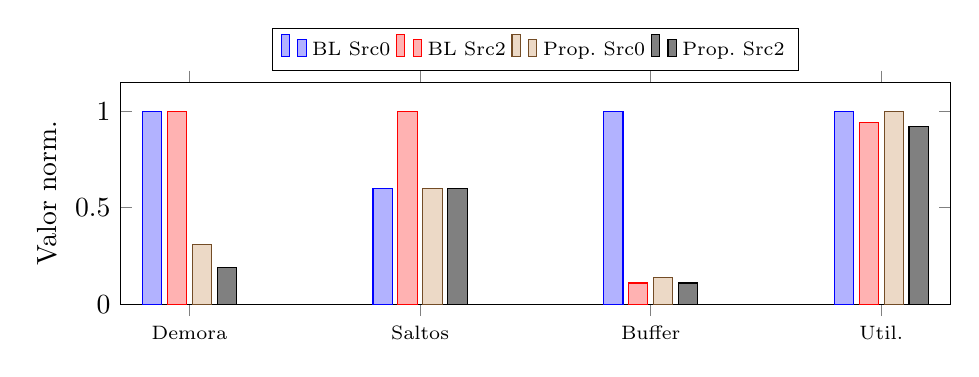
\begin{tikzpicture}
    \begin{axis}[
      width=\linewidth,
      height=4.4cm,
      ybar,
      bar width=7pt,
      ymin=0, ymax=1.15,
      symbolic x coords={Demora,Saltos,Buffer,Util.},
      xtick=data,
      x tick label style={font=\scriptsize},
      ylabel={Valor norm.},
      title={\scriptsize Caso~1: métricas normalizadas por fuente},
      legend style={font=\scriptsize, at={(0.5,1.05)},
                    anchor=south, legend columns=-1},
    ]
      % Baseline: Fuente0 y Fuente2 (normalizados sobre el máximo del baseline)
      % Delay: src0=53.25 src2=53.25 (similares), hops: src0=3 src2=5
      % Buffer: node[0]=199, node[2]=~22; Util: node[0]=98%, node[2]=92%
      \addplot coordinates {
        (Demora,1.00)(Saltos,0.60)(Buffer,1.00)(Util.,1.00)};
      \addplot coordinates {
        (Demora,1.00)(Saltos,1.00)(Buffer,0.11)(Util.,0.94)};
      % Propuesto: Fuente0 y Fuente2
      % Delay: src0=16.76/53.25=0.315, src2=10.20/53.25=0.192
      % Hops: ambos 3 saltos → src0=0.60, src2=1.00 (sobre max 5)
      % Buffer: node[0].lnk[0]=27/199=0.136, node[2].lnk[1]=21/199=0.105
      % Util: node[0].lnk[0]=97.5/98=0.995, node[2].lnk[1]=90/98=0.918
      \addplot coordinates {
        (Demora,0.31)(Saltos,0.60)(Buffer,0.14)(Util.,1.00)};
      \addplot coordinates {
        (Demora,0.19)(Saltos,0.60)(Buffer,0.11)(Util.,0.92)};
      \legend{BL Src0, BL Src2, Prop.\ Src0, Prop.\ Src2}
    \end{axis}
  \end{tikzpicture}
  \caption{Métricas normalizadas del Caso~1 por fuente de origen.
           Valores normalizados sobre el máximo del baseline.
           La mejora en demora es notable; la utilización de enlace
           permanece alta porque cada flujo satura su propio enlace.}
  \label{fig:comparacion-c1}
\end{figure}

\subsubsection*{Caso 2}

La Tabla~\ref{tab:comparacion-c2} presenta la comparación completa de métricas para todos los valores de \texttt{interArrivalTime}, mientras que la Figura~\ref{fig:comparacion-delay-c2} ilustra la evolución de la demora media E2E en ambos algoritmos.

Como se puede observar en los datos empíricos, en escenarios de saturación extrema (IAT de 0.5 a 2\,s), ambas estrategias sufren demoras altísimas y cuellos de botella severos. Sin embargo, incluso en ese régimen crítico, el algoritmo propuesto logra un mejor desempeño general, llegando a duplicar la tasa de entrega efectiva (R/E ratio) respecto al baseline (pasando del 14.0\% al 28.0\% para un IAT de 1\,s).

La divergencia de rendimiento se vuelve drástica en el rango de tráfico moderado (IAT entre 4 y 6\,s). En este punto, mientras el algoritmo baseline mantiene una demora media de casi 40\,s y colas largas, el algoritmo propuesto logra descongestionar la red, reduciendo la ocupación máxima a solo 8 paquetes y desplomando la demora a 6.58\,s (una mejora del 83.5\%). Como evidencia la curva de la Figura~\ref{fig:comparacion-delay-c2}, el nuevo esquema logra desplazar el umbral de estabilidad empírico de la red: mientras el baseline recién se estabiliza a los 8\,s, la nueva estrategia alcanza un estado estacionario seguro a los 6\,s.

\begin{table*}[!t]
  \centering
  \caption{Comparación Caso~2: baseline vs.\ algoritmo propuesto para
           distintos \texttt{interArrivalTime}. BufMáx corresponde a
           \texttt{node[6].lnk[0]} (cuello de botella del baseline) y
           \texttt{node[4].lnk[1]} (cuello del propuesto).}
  \label{tab:comparacion-c2}
  \begin{tabular}{@{}rrrrrrrrr@{}}
    \toprule
    \multirow{2}{*}{\textbf{IAT (s)}} &
    \multicolumn{2}{c}{\textbf{Demora media (s)}} &
    \multirow{2}{*}{\textbf{Mej.\,(\%)}} &
    \multicolumn{2}{c}{\textbf{BufMáx (pkts)}} &
    \multicolumn{2}{c}{\textbf{R/E ratio}} &
    \multirow{2}{*}{\textbf{¿Est.?}} \\
    \cmidrule(lr){2-3}\cmidrule(lr){5-6}\cmidrule(lr){7-8}
    & \textbf{Base} & \textbf{Prop.} & &
      \textbf{Base} & \textbf{Prop.} &
      \textbf{Base} & \textbf{Prop.} & \\
    \midrule
    0.5 & 75.09 & 75.01 &  0.1\% & 421 & 421 & 0.071 & 0.141 & No \\
    1   & 65.92 & 63.87 &  3.1\% & 218 & 218 & 0.140 & 0.280 & No \\
    2   & 56.52 & 42.93 & 24.0\% & 102 &  99 & 0.274 & 0.544 & No \\
    4   & 39.99 &  6.58 & 83.5\% &  50 &   8 & 0.536 & 0.951 & No/Borde \\
    6   & 17.49 &  2.98 & 82.9\% &  25 &   3 & 0.836 & 0.996 & Sí \\
    8   &  6.19 &  2.72 & 56.1\% &   4 &   3 & 0.970 & 0.988 & Sí \\
    \bottomrule
  \end{tabular}
\end{table*}

La Figura~\ref{fig:comparacion-delay-c2} muestra la evolución de la demora
media con ambos algoritmos.

\begin{figure}[!t]
  \centering
  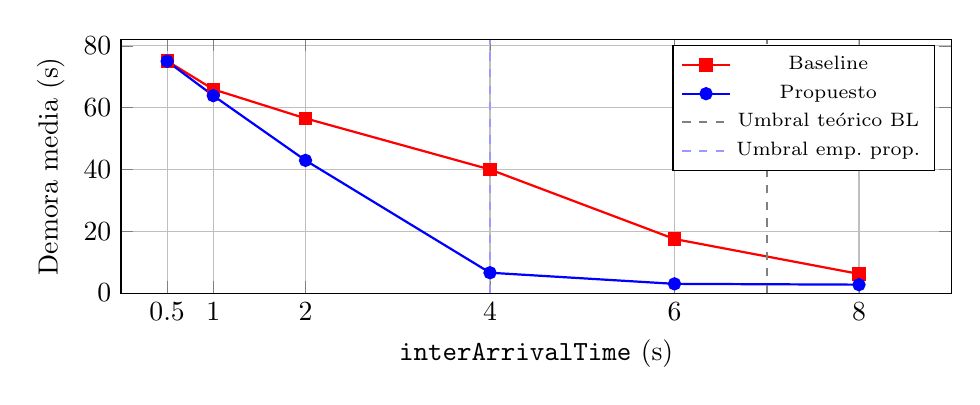
\begin{tikzpicture}
    \begin{axis}[
      width=\linewidth,
      height=4.8cm,
      xlabel={\texttt{interArrivalTime} (s)},
      ylabel={Demora media (s)},
      xmin=0, xmax=9, ymin=0, ymax=82,
      grid=major,
      xtick={0.5,1,2,4,6,8},
      legend style={font=\scriptsize, at={(0.98,0.98)}, anchor=north east},
    ]
      \addplot[thick, red, mark=square*, mark size=2pt] coordinates {
        (0.5,75.09)(1,65.92)(2,56.52)(4,39.99)(6,17.49)(8,6.19)
      };
      \addlegendentry{Baseline}
      \addplot[thick, blue, mark=*, mark size=2pt] coordinates {
        (0.5,75.01)(1,63.87)(2,42.93)(4,6.58)(6,2.98)(8,2.72)
      };
      \addlegendentry{Propuesto}
      \addplot[thick, gray, dashed] coordinates {(7,0)(7,82)};
      \addlegendentry{Umbral teórico BL}
      \addplot[thick, blue!40, dashed] coordinates {(4,0)(4,82)};
      \addlegendentry{Umbral emp.\ prop.}
    \end{axis}
  \end{tikzpicture}
  \caption{Demora media E2E vs.\ \texttt{interArrivalTime} para ambos
           algoritmos. El algoritmo propuesto alcanza la estabilidad
           empíricamente a partir de IAT\,=\,6\,s frente a IAT\,=\,8\,s
           del baseline.}
  \label{fig:comparacion-delay-c2}
\end{figure}

\begin{figure}[!t]
  \centering
  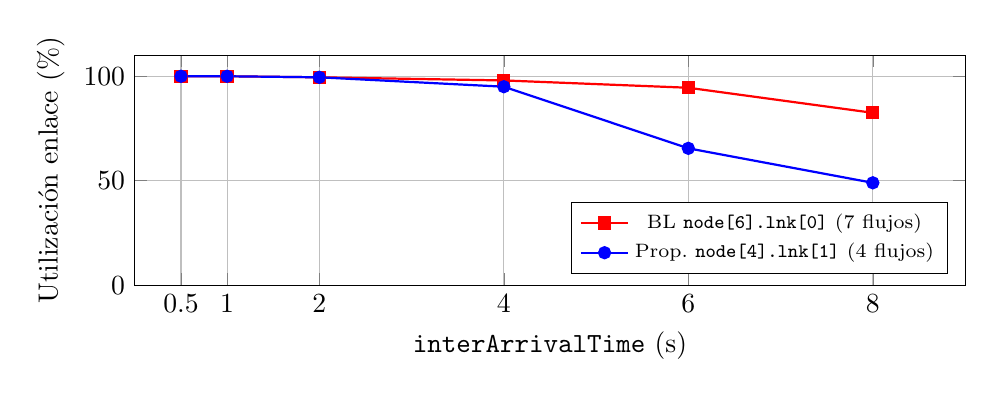
\begin{tikzpicture}
    \begin{axis}[
      width=\linewidth,
      height=4.5cm,
      xlabel={\texttt{interArrivalTime} (s)},
      ylabel={Utilización enlace (\%)},
      xmin=0, xmax=9, ymin=0, ymax=110,
      grid=major,
      xtick={0.5,1,2,4,6,8},
      legend style={font=\scriptsize, at={(0.98,0.05)}, anchor=south east},
    ]
      \addplot[thick, red, mark=square*, mark size=2pt] coordinates {
        (0.5,100.0)(1,100.0)(2,99.5)(4,98.0)(6,94.5)(8,82.5)
      };
      \addlegendentry{BL \texttt{node[6].lnk[0]} (7 flujos)}
      \addplot[thick, blue, mark=*, mark size=2pt] coordinates {
        (0.5,100.0)(1,100.0)(2,99.5)(4,95.0)(6,65.5)(8,49.0)
      };
      \addlegendentry{Prop.\ \texttt{node[4].lnk[1]} (4 flujos)}
    \end{axis}
  \end{tikzpicture}
  \caption{Utilización del enlace cuello de botella en cada algoritmo.
           El propuesto reduce la carga máxima de 7 a 4 flujos
           concentrados, lo que adelanta el umbral de estabilidad.}
  \label{fig:comparacion-util-c2}
\end{figure}

\subsection{Discusión de resultados}

\subsubsection*{¿Cuánto mejoran las métricas y por qué?}

Las mejoras son drásticas en el régimen de tráfico moderado. Con
IAT\,=\,4\,s la demora cae un \textbf{83.5\%} (de 39.99\,s a 6.58\,s)
y el buffer máximo se reduce de 50 a 8 paquetes. La causa es estructural:
el baseline acumula \textbf{7 flujos} en un único enlace
(\texttt{node[6].lnk[0]}), mientras que el algoritmo propuesto
distribuye el tráfico simétricamente en ambas direcciones del anillo.
El nuevo cuello de botella, \texttt{node[4].lnk[1]}, concentra solo
\textbf{4 flujos} (los nodos 1, 2, 3 y 4 que van en sentido horario),
lo que reduce la utilización máxima de 98\,\% a 49\,\% con IAT\,=\,8\,s
(Fig.~\ref{fig:comparacion-util-c2}).

Otro indicador clave es el ratio R/E: con IAT\,=\,4\,s el baseline
entrega solo el 53.6\,\% de los paquetes generados, mientras que el
algoritmo propuesto entrega el 95.1\,\%. La estabilidad práctica
se alcanza a partir de \textbf{IAT\,=\,6\,s} en el nuevo algoritmo
(R/E\,=\,0.996, buffer máx.\,=\,3), un umbral un 14\,\% menor que el
del baseline (IAT\,=\,8\,s).

El nuevo umbral teórico puede estimarse como:

\begin{equation}
  \rho_{\mathrm{prop}} = \frac{4}{\mathrm{IAT}} < 1
  \quad \Rightarrow \quad \mathrm{IAT} > 4\,\mathrm{s}
  \label{eq:umbral-nuevo}
\end{equation}

\noindent donde 4 es el número de flujos en el enlace más cargado
(\texttt{node[4].lnk[1]}). Los datos confirman que con IAT\,=\,4\,s la
red está en el límite (R/E\,=\,0.951, util.\,=\,95\,\%) y con
IAT\,=\,6\,s ya es estable, consistente con la predicción teórica.

\subsubsection*{¿Hay loops de enrutamiento?}

No se observaron loops de enrutamiento en ninguna de las simulaciones.
El algoritmo garantiza ausencia de loops por construcción: dado que cada
nodo calcula la distancia mínima en ambos sentidos y elige la interfaz
correspondiente al camino más corto, el destino siempre se acerca en
cada salto. En un anillo, esto implica que el paquete viaja
monótonamente en una sola dirección hasta llegar al destino, sin
posibilidad de dar vueltas. El máximo de saltos observado fue 4 (la
distancia máxima en un anillo de 8 nodos), consistente con la ausencia
de loops.

\subsubsection*{¿Qué pasaría con muchos más nodos?}

El algoritmo propuesto escala mejor que el baseline. En un anillo de
$N$ nodos, el baseline siempre acumula todos los flujos en un único
enlace adyacente al destino ($N-1$ flujos), con umbral de estabilidad
$\mathrm{IAT} > N-1$. El algoritmo propuesto distribuye los flujos
simétricamente: el enlace más cargado acumula $\lceil N/2 \rceil$
flujos (los nodos del lado más largo), con umbral
$\mathrm{IAT} > \lceil N/2 \rceil$. Para $N$ grande, la mejora en
el umbral de estabilidad es del orden de $2\times$. Sin embargo, la
fase de descubrimiento (Hello\,+\,Echo) requiere que el paquete Hello
complete una vuelta completa al anillo, lo que implica un retardo de
convergencia de $O(N)$ antes de que el ruteo óptimo esté disponible.
Durante ese período, los paquetes de datos que llegan se reenvían por
\texttt{lnk[0]} (fallback al baseline). Para $N$ muy grande, este
tiempo de convergencia puede ser significativo.

\subsubsection*{¿Qué sucede si cae un nodo?}

El baseline no es tolerante a fallos: si cae cualquier nodo del único
camino posible hacia el destino, los paquetes se pierden
indefinidamente. El algoritmo propuesto tampoco es tolerante a fallos
en su implementación actual: la tabla de ruteo se construye una sola
vez al inicio mediante el Hello y no se actualiza dinámicamente. Si
un nodo cae después de la fase de descubrimiento, los paquetes que
deban transitar por él seguirán siendo enviados en esa dirección y se
perderán. Una extensión natural sería incorporar mensajes de Hello
periódicos para detectar caídas y recalcular las rutas, similar al
mecanismo de \emph{keepalive} utilizado en protocolos como OSPF o RIP.

\section{Conclusiones}
\label{sec:conclusiones}

En este trabajo se evaluó el rendimiento de una red en topología de anillo bajo distintos escenarios de carga. El algoritmo original (baseline) demostró ser estructuralmente ineficiente al rutear todo el tráfico en una única dirección, lo que generó cuellos de botella severos (ej. colas de 199 paquetes en el Caso 1, ver Tabla~\ref{tab:caso1}) y un umbral de saturación prematuro (IAT $\leq$ 7\,s en el Caso 2, Fig.~\ref{fig:caso2-estabilidad}) debido a la acumulación innecesaria de flujos en un solo enlace.

Para resolver estas limitaciones, se diseñó e implementó un algoritmo de enrutamiento basado en la distancia mínima, el cual descubre el tamaño de la topología de forma autónoma mediante el intercambio de paquetes \texttt{hello} y \texttt{echo}. Los resultados obtenidos confirmaron una mejora sustancial: al balancear la carga utilizando ambos sentidos del anillo, las demoras medias se redujeron hasta un 83.5\% (Tabla~\ref{tab:comparacion-c2}) y la red logró mantener la estabilidad frente a mayores tasas de inyección de tráfico (IAT $\geq$ 6\,s, Fig.~\ref{fig:comparacion-delay-c2}). Además, el diseño garantizó matemáticamente la ausencia de bucles de enrutamiento.

Como trabajo futuro, la principal oportunidad de mejora detectada es la tolerancia a fallos. Actualmente, la fase de descubrimiento se ejecuta una única vez; incorporar un mecanismo de actualización dinámica (mensajes \emph{keepalive} periódicos) permitiría recalcular las rutas ante la caída inesperada de un nodo o enlace, dotando a la red de resiliencia.

\section*{Agradecimientos}

Agradecemos a la cátedra de Redes y Sistemas Distribuidos por su constante acompañamiento y por la provisión de material original que nos prepara de manera integral, tanto para los desafíos de la industria como para el ámbito científico. Valoramos profundamente su compromiso con nuestro crecimiento personal y profesional, esfuerzo que resulta destacable y necesario frente al actual contexto de desfinanciamiento y dificultades presupuestarias que atraviesa la universidad pública.

% Bibliografía mínima de ejemplo
\begin{thebibliography}{99}

\bibitem{omnetpp}
A. Varga and R. Hornig,
``OMNeT++,''
in \emph{Proc.\ Int.\ Conf.\ Simulation Tools and Techniques (Simutools)}, 2008.

\bibitem{kickstarter}
Cátedra de Redes y Sistemas Distribuidos,
``Laboratorio 4: kickstarter OMNeT++,''
FaMAF/UNC, 2026.

\bibitem{tanenbaum}
A. S. Tanenbaum and D. J. Wetherall,
\emph{Computer Networks}, 5th ed.
Upper Saddle River, NJ, USA: Prentice Hall, 2011.

\end{thebibliography}

\end{document}